\documentclass[french,a4paper,12pt]{article} 
\usepackage[utf8]{inputenc}
\usepackage[T1]{fontenc}
\usepackage[a4paper,left=2cm,right=2cm,top=2cm,bottom=2cm]{geometry}
\usepackage{mathtools}
\usepackage[french]{babel}
\usepackage{perpage}
\usepackage{libertine}
\usepackage{blindtext}
\usepackage{babel}
\usepackage[pdftex]{graphicx}
\usepackage[rightcaption]{sidecap}
\usepackage{lmodern}
\usepackage{url}
\usepackage{algorithm}
\usepackage{algorithmic}
\setlength{\parindent}{0cm}
\setlength{\parskip}{1ex plus 0.5ex minus 0.2ex}
\newcommand{\hsp}{\hspace{20pt}}
\newcommand{\HRule}{\rule{\linewidth}{0.5mm}}
\selectlanguage{french}
\title{Le Boosting en Machine Learning} % le titre de l'article
\author{Metango Kenfack Cathy Judith} 
\usepackage{caption,subcaption}
\tracinglostchars=2
\usepackage{iftex}
\pagestyle{plain}
\usepackage[authoryear]{natbib}
\ifTUTeX
  \usepackage{fontspec}
\else
  \usepackage[T1]{fontenc}
  \usepackage[utf8]{inputenc} % The default since 2018
  \DeclareUnicodeCharacter{200B}{{\hskip 0pt}}
\fi
\usepackage[]{tocbibind}
 \DeclareUnicodeCharacter{202F}{\,}

\begin{document}
\begin{titlepage}
  \begin{sffamily}
  \begin{center}
     
\includegraphics[scale=0.25]{logoulb.JPG}~\\[1.5cm]

    \textsc{\bfseries \LARGE Université Libre de Bruxelles }\\[0.5cm]
    \textsc{\Large Faculté de Lettres, Traduction et Communication}\\[6cm]

    % Title
    \HRule \\[0.4cm]
    { \huge \bfseries Le Boosting en Machine Learning\\[0.4cm] }

    \HRule \\[4cm]
    % Author and supervisor
    \begin{minipage}{0.4\textwidth}
      \begin{flushleft} \large
        Metango Kenfack Cathy \\

        
      \end{flushleft}
    \end{minipage}
    \begin{minipage}{0.4\textwidth}
      \begin{flushright} \large
        \emph{Travail réalisé sous la direction de DE VALERIOLA Sébastien dans le cadre du cours d'Architecture des Systèmes d'information (M-STIC-B540)} 
      \end{flushright}
    \end{minipage} \\ [2cm]

    \vfill

    % Bottom of the page
    {\large {} Année académique 2022-2023}

  \end{center}
  \end{sffamily}
\end{titlepage}


 %%fin de la parge de garde 
 \begin{center}
 \tableofcontents
 \end{center}
\newpage



\section{Introduction}
<<<<<<< HEAD
\quad Le thème soumis à notre étude est celui du Boosting en machine Learning. L’apprentissage automatique est une discipline qui permet de donner à un ordinateur la capacité d’apprendre à partir des données pour résoudre une tache qui implique généralement les prédictions, Il s’agit d’un sous-domaine de l'intelligence artificielle, qui est définie au sens large comme la capacité d'une machine à imiter le comportement humain intelligent \citep{kubat}. Les systèmes d'intelligence artificielle sont utilisés pour exécuter des tâches complexes d'une manière similaire à la façon dont les humains résolvent les problèmes. L'apprentissage automatique utilisent pour ce fait des méthodes pour apprendre des informations à partir des données sans modèle de référencé prédéterminé, Il existe de ce faites plusieurs méthodes de machine Learning parmi lesquelles l’algorithme de boosting. Le boosting est un algorithme de machine Learning permettant \ de réduire les erreurs dans l’analyse prédictive des données. C’est une méthode d’ensemble Learning c’est a dire elle crée un modèle fort a partir d’un certain nombre de modèles faibles cela en demandant a chaque model de corriger les erreurs de son prédécesseur : les faiblesses des uns sont compensées par les forces des autres. L étude de ce projet porte sur cette notion qu’est le BOOSTING. Pour mener a bien cette étude nous aborderons plusieurs points à savoir la Définition du machine Learning et du boosting  d'une part et d'autre part donner l’importance du boosting, présenter le principe et fonctionnement du boosting et enfin donner  un exemple d’algorithme du boosting à savoir Adaboost. 
=======
\quad Le thème soumis à notre étude est celui du Boosting en machine Learning. L’apprentissage automatique est une discipline qui permet de donner à un ordinateur la capacité d’apprendre à partir des données pour résoudre une tache qui implique généralement les prédictions, Il s’agit d’un sous-domaine de l'intelligence artificielle, qui est définie au sens large comme la capacité d'une machine à imiter le comportement humain intelligent. Les systèmes d'intelligence artificielle sont utilisés pour exécuter des tâches complexes d'une manière similaire à la façon dont les humains résolvent les problèmes. L'apprentissage automatique utilisent pour ce fait des méthodes pour apprendre des informations à partir des données sans modèle de référencé prédéterminé, Il existe de ce faites plusieurs méthodes de machine Learning parmi lesquelles l’algorithme de boosting. Le boosting est un algorithme de machine Learning permettant \ de réduire les erreurs dans l’analyse prédictive des données. C’est une méthode d’ensemble Learning c’est a dire elle crée un modèle fort a partir d’un certain nombre de modèles faibles cela en demandant a chaque model de corriger les erreurs de son prédécesseur : les faiblesses des uns sont compensées par les forces des autres. L étude de ce projet porte sur cette notion qu’est le BOOSTING. Pour mener a bien cette étude nous aborderons plusieurs points à savoir la Définition du machine Learning et du boosting  d'une part et d'autre part donner l’importance du boosting, présenter le principe et fonctionnement du boosting et enfin donner  un exemple d’algorithme du boosting à savoir Adaboost. 
>>>>>>> b05b784cd2e20090e2301b6dc709dcdfaf091d7c




\newpage
\section{Machine Learning}
\subsection{Définition}
<<<<<<< HEAD
\quad Notre camarade de classe a du mal à faire une différence entre le citron et la mandarine avec suffisamment de précision pour la reconnaitre dans un supermarché. Mais si nous lui montrons quelques-unes des  photos de ces fruits, il repérera immédiatement les traits révélateurs dont il a besoin. Comme on dit, une image, un exemple, vaut mille mots supposons ici que notre ami c’est notre machine et qu’on aimerait apprendre à la machine à distinguer les citrons des mandarines. Plutôt que de coder une machine avec des images représentatifs des citrons et mandarines, nous pouvons plutôt programmer la machine pour apprendre à les distinguer grâce à une expérience répétée avec les citrons et les mandarines réelles. C’est ça le machine Learning donner la capacite à un ordinateur d’apprendre à partir des données.
=======
\quad Notre camarade de classe a du mal à faire une différence entre le citron et la mandarine avec suffisamment de précision pour la reconnaitre dans un supermarché. Mais si nous lui montrons quelques-unes de ses photos, il repérera immédiatement les traits révélateurs dont il a besoin. Comme on dit, une image, un exemple, vaut mille mots supposons ici que votre ami c’est votre machine et qu’on aimerait apprendre à la machine à distinguer les citrons des mandarines. Plutôt que de coder une machine avec des images représentatifs des citrons et mandarines, nous pouvons plutôt programmer la machine pour apprendre à les distinguer grâce à une expérience répétée avec les citrons et les mandarines réelles. C’est ça le machine Learning donner la capacite à un ordinateur d’apprendre à partir des données.
>>>>>>> b05b784cd2e20090e2301b6dc709dcdfaf091d7c

\quad Incapables de définir certains objets ou concepts avec suffisamment de précision, nous voulons les transmettre à la machine au moyen d'exemples\citep{elnaqa}. Pour que cela fonctionne, cependant, l'ordinateur doit avoir la capacité de convertir les exemples fournis par l’humain pendant l’apprentissage en connaissances. Une fois que cette phase d’apprentissage est faite, on peut faire des prédictions c’est à dire produire une réponse correcte sur les données similaires mais sur lesquelles le programme n’a pas été entrainée.   D'où l’intérêt pour les algorithmes d’apprentissage automatique, le sujet de ce manuel.

<<<<<<< HEAD
\quad Le machine Learning est donc une branche évolutive des algorithmes ayant pour but d’imiter la capacite humaine. Elle s’appuie sur les  notions de déférentes disciplines telles que informatique, l’intelligence artificielle, les probabilités  statistiques, et la psychologie.  Elle a montré son importance et elle est appliqué dans plusieurs domaines varié de la vie tel qu’en finance pour la prédiction du chiffre d’affaires, la détection de fraude, en transport pour la prédiction du nombre d’accident en politique pour la prédiction de résultat, en biologie, en divertissement, en marketing , en médecine , en biomédecine, en physique médicale et bien encore.
=======
\quad Le machine Learning est donc une branche évolutive des algorithmes ayant pour but d’imiter la capacite humaine. Elle s’appuie sur notions de déférentes disciplines telles que informatique, l’intelligence artificielle, les probabilités et statistiques, la psychologie.  Elle a montré son importance et elle est applique dans plusieurs domaines varie de la vie tel qu’en finance pour la prédiction du chiffre d’affaires, la détection de fraude, en transport pour la prédiction du nombre d’accident en politique pour la prédiction de résultat, en biologie, en divertissement, en marketing , en médecine , en biomédecine, en physique médicale et bien encore.
>>>>>>> b05b784cd2e20090e2301b6dc709dcdfaf091d7c




\subsection{ fonctionnements du machine Learning : apprendre à partir des données }

<<<<<<< HEAD
\quad Les machines pour qu’elles apprennent ont besoin des données (images, sons, textes, vidéos, prix d’une maison). Ce processus en apprentissage automatique est appelé expérience. Après avoir données ces donnes à la machine on doit par suite préciser la tâche  quelle doit réaliser (catégoriser les images, prédire le prix d’une maison, prédire le chiffre d’affaires). En fonction de la tache quelle a appris nous devons à la fin évaluer son apprentissage pour mesurer sa performance. Il existe donc pour ce fait des algorithmes d’apprentissages. Le machine Learning regroupe trois grandes familles d’algorithme d’apprentissage : apprentissage supervisé, apprentissage non supervisé et apprentissage semi supervisé. En fonction du type d’apprentissage nous avons plusieurs algorithmes, mais comme énoncé plus haut nous parlerons d’algorithme de boosting qui est un algorithme d’apprentissage supervisé\citep{elnaqa}. 
=======
\quad Les machines pour qu’elles apprennent ont besoin des données (images, sons, textes, vidéos, prix d’une maison). Ce processus en apprentissage automatique est appelé expérience. Après avoir donné ces donnes à la machine on doit par suite préciser la tâche  quelle doit réaliser (catégoriser les images, prédire le prix d’une maison, prédire le chiffre d’affaires). En fonction de la tache quelle a appris nous devons à la fin évaluer son apprentissage pour mesurer sa performance. Il existe donc pour ce fait des algorithmes d’apprentissages. Le machine Learning regroupe trois grandes familles d’algorithme d’apprentissage : apprentissage supervisé, apprentissage non supervisé et apprentissage semi supervisé. En fonction du type d’apprentissage nous avons plusieurs algorithmes, mais comme énoncé plus haut nous parlerons d’algorithme de boosting qui est un algorithme d’apprentissage supervisé\citep{elnaqa}. 
>>>>>>> b05b784cd2e20090e2301b6dc709dcdfaf091d7c

\section{Algorithme de Boosting}
\quad 
Nous présentons dans cette section le boosting et son fonctionnement et par la suite nous  illustrons les differents types d'algorithme du boosting.

 \subsection{Enjeux : Pourquoi le boosting est t'il utilisé}

\quad Avec le development de la technologie , le progrès dans les divers domaines tel que le marketing , la santé , les finance , etc…, il est necessaires de développer des techniques d'apprentissage automatique plus complexes et plus avancées\citep{educa}. 

\quad Le boosting est une technique qui peut etre utilisée pour resoudre des problemes complexes , basés sur des données et le monde réel.
Supposons qu'on veux   créer un modèle pour un ensemble de données d'images contenant des images de chats et de chiens et que nous voulons classer ces images en deux classes différentes. Nous allons pour cela  commencer par identifier les images en fonction de certaines règles, telles que les éléments suivants : 
\begin{enumerate} 
    \item La photo a des oreilles pointues : chat
    \item L'image est un œil en forme de chat : chat
    \item L'image a de grands membres : chien
    \item L'image a des griffes aiguisees : chat
     \item L'image a une structure de bouche plus large : chien
\end{enumerate}  

\quad En effet , les prédictions de chacun de ces apprenants faibles peuvent être combinées avec une règle de majorité ou une moyenne pondérée pour rendre les prédictions plus précises. Cela en fait de solides modèles d'apprentissage.
Dans lexemple ci dessus, nous avons defini 5 classificateurs faibles et  la majorite de ces regles (3 classificateurs sur 5 predisent l'image comme un chat) nous donne la prediction que l’image est un chat. On conclus que notre sortie est un chat. 

\subsection{Définition}

 \quad Le boosting est une technique d’ensemble général qui crée un apprenant fort à partir d’un certains nombre d’apprenant faibles. Cela se fait en construisant un modèle à partir des données d’apprentissage puis en créant un deuxième modèle qui tente de corriger les erreurs du modèle precédent. 

\subsection{ Les techniques d'ensemble learning}
<<<<<<< HEAD

\quad En regroupant un ensemble de modèles , on obtiens une meilleurs performance que lorsqu’on utilise nos modèles chacun de leur cote. Cette méthode est basé sur le concept "The wisdom of the crowd" qui est un phenomene lié à la loi des grands nombres qui fait q'une foule d’individus à souvent plus raison qu’un expert tout seul  à condition que la foule soit grande et diversifiée (les modèles doivent etres différent, construit sur des données différentes ou avec des algorithmes d’apprentissage différents)et compétentes. En apprentissage automatique on peu  utiliser ce concept pour creéer un ensemble de modèles qui surpassent les performances des meilleures modèles de machine d’apprentissage au monde\citep{ens}. Pour cela on distingue 3 grandes techniques qui sont : le Bagging , le Boosting et le Stacking.




\textbf{Le Boosting} 
\quad Ici, les apprenants faibles sont générés séquentiellement  , en demandant à chaque modèle de corriger les erreurs de son predécesseur, on n’a donc toujours un nouvel algorithme formé sur les mauvaises pr2dictions faites précédemment\citep{ens}. En attribuant des poids plus élevés aux échantillons précédemment mal classés, les performances du modèle sont améliorées. Un exemple de boosting est l'algorithme AdaBoost.
=======

\quad En regroupant un ensemble de modeles , on obtiens ume meilleurs performance que lorsqu’on utilise nos modèles chacun de leur cote. Cette methode est base sur le concept The wisdom of the crowd qui est un phenomene lie a la loi des grands nombres qui fait qune foule d’individus a souvent plus raison qu’un expert tout seul  a condition que la foule soit grande et diversifieée (les modèles doivent etres différent, construit sur des données différents ou avec des algorithms d’apprentissage différents)et compétente. En apprentissage automatique on peu  utiliser ce concept pour creer un ensemble de modeles qui surpassent les performances des meilleures modeles de machine d’apprentissage au monde\citep{ens}. Pour cela on distingue 3 grandes techniques qui sont : le Bagging , le Boosting et le Stacking.




\textbf{le Boosting} 
\quad Ici, les apprenants faibles sont générés séquentiellement  , en demandant à chaque modèle de corriger les erreurs de son predécesseur, on n’a donc toujours un nouvel algorithme formé sur les mauvaises predictions faites précédemment\citep{ens}. En attribuant des poids plus élevés aux échantillons précédemment mal classés, les performances du modèle sont améliorées. Un exemple de boosting est l'algorithme AdaBoost.
>>>>>>> b05b784cd2e20090e2301b6dc709dcdfaf091d7c

\textbf{Le Bagging} 
\quad les apprenants faibles sont produits parallèlement. Ici , les données sont échantillonnées (le boosstrapping) et on obtenir un ensemble de modèles diversifiés en entrenant sur une portion aleatoire de données chaque modèle. La prediction finale est la moyenne des predictions de chaque modèles qui ont été préalablement obtenus. 

\textbf{Le Stacking}
<<<<<<< HEAD
\quad cette technique consiste à entrainer plusieurs modèles différents avec les meme données puis utiliser les resultats des différents modèles  sur un modèle final qui donne la prediction finale. Elle permet d'entrainer un modèle d ‘apprentissage à reconnaitre qui a tort et qui a raison dans un ensembles de modèles, ceci améliore encore plus la performance générale. 
=======
\quad cette technique consiste à entrainer plusieurs modèles différents avec les meme données puis utiliser les resultats des différents modèles  sur un modèle final qui donne la prediction finale. Elle permet entrainer un modèle d ‘apprentissage à reconnaitre qui a tort et qui a raison dans un ensembles de modèles, ceci améliore encore plus la performance générale. 
>>>>>>> b05b784cd2e20090e2301b6dc709dcdfaf091d7c

\quad Bien que ces trois modèles sont très important pour la prédiction des problèmes complexes, nous allons nous focalisé sur les techniques du boosting.


 

\subsection{Fonctionnement du boosting}
<<<<<<< HEAD
\quad Le principe de base de l'algorithmes  boosting est de générer plusieurs apprenants faibles et de combiner leurs prédictions pour former un apprenant fort. Ces apprenants faibles sont générés en appliquant des algorithmes d'apprentissage automatique de base à différentes distributions de l'ensemble de données\citep{educa}. Ces algorithmes génèrent des règles faibles à chaque itération. Après quelques itérations, les apprenants faibles sont combinés en apprenants forts qui prédisent des résultats plus précis.
=======
\quad Le principe de base de algorithmes de boosting est de générer plusieurs apprenants faibles et de combiner leurs prédictions pour former un apprenant fort. Ces apprenants faibles sont générés en appliquant des algorithmes d'apprentissage automatique de base à différentes distributions de l'ensemble de données.\citep{educa} Ces algorithmes génèrent des règles faibles à chaque itération. Après quelques itérations, les apprenants faibles sont combinés en apprenants forts qui prédisent des résultats plus précis.
>>>>>>> b05b784cd2e20090e2301b6dc709dcdfaf091d7c



\textbf{étape 1}
 \quad L'algorithme de base lit les données et attribue des poids égaux à chaque observation d'échantillon de données. Puis algorithme de base faire des predictions pour chacun de ces échantillons.
 
 \textbf{étape 2}
 \quad L’algorithme identifie les prédictions incorrectes faites par l'apprenants de base. À l'itération suivante, ces prédictions erronées sont attribuées à l'apprenant de base suivant avec des poids plus élevés pour ces prédictions erronées.

 
 \textbf{étape 3}
\quad on répète l'étape 2 jusqu'à ce que l'algorithme puisse apprendre correctement.
Par conséquent, l'objectif principal du boosting est de se concentrer davantage sur les prédictions erronées.

\quad Maintenant que nous connaissons comment fonctionne l’algorithme de boosting, intéressons-nous maintenant aux différents types de algorithme de boosting. Mais avant nous présenterons des Forces  et Faiblesses de celui ci.



 \begin{center}
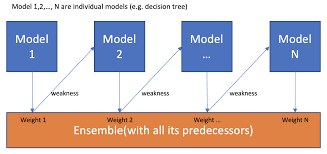
\includegraphics[scale=1]{boosting definition.png}
\begin{figure}[h]
\caption{Présentation de la technique du Boosting}
\end{figure}
\end{center}
\subsection{Les forces et Faiblesses du Boosting}


\subsubsection{ Les forces de l'algorithme de Boosting}

\quad Le boosting offrent plusieurs avantages.



\textbf{ Facile à implémenter }


<<<<<<< HEAD
\quad  grâce à ces algorithmes faciles à comprendre et à interpréter qui apprennent de leurs erreurs, Ces algorithmes ne nécessitent aucun prétraitement des données et disposent de routines intégrées pour gérer les données manquantes\citep{AWS}. De plus, la plupart des langages ont des bibliothèques intégrées pour implémenter des algorithmes de boosting avec de nombreux paramètres pour affiner les performances.
=======
\quad  grâce a ces algorithmes faciles à comprendre et à interpréter qui apprennent de leurs erreurs, Ces algorithmes ne nécessitent aucun prétraitement des données et disposent de routines intégrées pour gérer les données manquantes\citep{AWS}. De plus, la plupart des langages ont des bibliothèques intégrées pour implémenter des algorithmes de boosting avec de nombreux paramètres pour affiner les performances.
>>>>>>> b05b784cd2e20090e2301b6dc709dcdfaf091d7c



\textbf{Reduction des biais }



\quad Le biais est la présence d'incertitude ou d'imprécision dans les résultats d'apprentissage automatique. Un algorithme de renforcement combine plusieurs apprenants faibles de manière itérative pour améliorer itérativement une observation. Cette approche permet d'atténuer les biais élevés communs aux modèles d'apprentissage automatique.




\textbf{Efficacité de calcul }


\quad Les algorithmes de boosting donnent la priorité aux fonctionnalités qui augmentent la précision des prédictions pendant l'entraînement. Ils permettent de réduire les attributs de données et de traiter efficacement de grands ensembles de données. Les algorithmes de boost donnent la priorité aux fonctionnalités qui augmentent la précision des prédictions pendant l'entraînement. Ils permettent de réduire les attributs de données et de traiter efficacement de grands ensembles de données.

\quad Malgré les forces de cet algorithme, elle présente néanmoins des faiblesses. 


\subsubsection{Les faiblesses de l'algorithme de boosting}

\textbf{Vulnérabilité aux données aberrantes }

\quad Les modèles de boost sont sujets aux valeurs aberrantes ou aux valeurs de données qui diffèrent du reste de l'ensemble de données. Comme chaque modèle tente de corriger les bogues du modèle précédent, les valeurs aberrantes peuvent grandement fausser les résultats\citep{AWS}.


\textbf{Implémentation en temps réel}

\quad Le boosting peut être difficile à utiliser pour les implémentations en temps réel car l'algorithme est plus complexe que les autres processus. Les techniques de boosting sont très adaptables. Cela vous permet d'utiliser différents paramètres de modèle qui affectent directement les performances du modèle.

\subsection{ Les différents types d'algorithme de boosting}


\quad Il existe trois façons principales d’effectuer le boosting.

\textbf{Boosting adaptatif }

\quad Adaptative Boosting (AdaBoost) a été l'un des premiers modèles de boosting développés. Il essaie de s'adapter et de s'autocorriger à chaque itération du processus de boosting.


<<<<<<< HEAD
\quad AdaBoost donne initialement à chaque ensemble de données un poids égal. Ensuite, ajuste automatiquement les poids des points de données après chaque itération. puis augmente le poids des éléments mal clasés pour les corriger au tour suivant. Ce processus est répété jusqu'à ce que le résidu, la différence entre la valeur réelle et la valeur prédite, tombe en dessous du seuil acceptable\citep{adaboost}.
=======
\quad AdaBoost donne initialement à chaque ensemble de données un poids égal. Ensuite, ajustez automatiquement les poids des points de données après chaque arbre de décision. Pesez les articles mal classés et corrigez-les pour le tour suivant. Ce processus est répété jusqu'à ce que le résidu, la différence entre la valeur réelle et la valeur prédite, tombe en dessous du seuil acceptable\citep{adaboost}.
>>>>>>> b05b784cd2e20090e2301b6dc709dcdfaf091d7c

\quad AdaBoost peut être utilisé avec de nombreux prédicteurs, mais il n'est généralement pas aussi sensible que d'autres algorithmes de boosting. Cette approche ne fonctionne pas bien lorsqu'il existe une corrélation entre les caractéristiques ou lorsque les données sont très dimensionnelles. 

\quad Dans l'ensemble, AdaBoost est un type de boosting approprié pour les problèmes de classification. 

\textbf{Le boosting de gradient}

\quad Gradient Boosting(GB), également connu sous le nom d’amplificateur de gradient, est similaire à AdaBoost en ce sens qu'il s'agit également d'une technique d'entraînement séquentielle.

<<<<<<< HEAD
\quad Contrairement à AdaBoost  GB ne donne pas de poids aux éléments mal classés,  le logiciel GB optimise la fonction de perte en générant des apprenants de base de manière séquentielle, de sorte que l'apprenant de base actuel est toujours plus éfficace que le précédent. Cette méthode essaie d'obtenir des résultats précis la première fois au lieu de corriger les erreurs en cours de route comme le fait AdaBoost\citep{educa}. Cela permet au logiciel GB de produire des résultats plus précis.
=======
\quad Contrairement à AdaBoost  GB ne donne pas de poids aux éléments mal classés,  le logiciel GB optimise la fonction de perte en générant des apprenants de base de manière séquentielle, de sorte que l'apprenant de base actuel est toujours plus efficace que le précédent. Cette méthode essaie d'obtenir des résultats précis la première fois au lieu de corriger les erreurs en cours de route comme le fait AdaBoost\citep{educa}. Cela permet au logiciel GB de produire des résultats plus précis.
>>>>>>> b05b784cd2e20090e2301b6dc709dcdfaf091d7c

\quad Le boosting de gradient est utile pour les problèmes de classification et de régression.




\textbf{Le boosting de gradient extreme}

\quad Extreme Gradient Boosting (XGBoost) améliore le boosting  de gradient de plusieurs manières en termes de vitesse de calcul\citep{mousa}. XGBoost utilise plusieurs cœurs du CPU, permettant un apprentissage parallèle pendant l’entrainement. Il s'agit d'un algorithme de boosting qui peut gérer de grands ensembles de données, ce qui le rend attractif pour les applications de Big Data. 

\quad Les principales fonctionnalités de XGBoost sont la parallélisation, le calcul distribuée, l'optimisation du cache et le traitement hors cœur.

\quad \quad Bien que ces trois algorithmes sont très important , nous allons nous focalisé sur algorithme Adaboost.

\section{Algorithme Adaboost}

\subsection{Présentation de l'algorithme. }

\begin{algorithm}
\caption{ algorithme AdaBoost.}\label{alg:cap}
\begin{algorithmic}

\REQUIRE D = {(x_1,y_1),\ldots,(x_m,y_m)} ou $x_i \in X$ , $y_i  \in [{-1,+1}]\\

\textbf{Initialisation:} $D_1(i)= \frac{1}{m} $  (initialisation de la repartision du poids)  $ \FOR{i=(1),\ldots,(m) } \\

\textbf{for} {i=(1),\ldots,(T): } ou T est le nombre de tours d'apprentissage  

\begin{enumerate}
\item Entraîner l'apprenant faible en utilisant la distribution D_t  

   
\item Obtenir l'hypothèse faible h_t :  \State $X $\rightarrow$  [{-1,+1}]



<<<<<<< HEAD


=======
>>>>>>> b05b784cd2e20090e2301b6dc709dcdfaf091d7c
\item Objectif : sélectionner $h_t$ pour minimiser l'erreur 


    \epsilon_t = \textbf{Pr}_i$\sim$D_t$[h_t(x_i) \ne y_i] = 
    \sum{(i:h_t(x_i)\ne y_i}) ^{} D_t(i)   
    $  (il s'agit du \% de mesure de l'erreur h_t)\\
    

              
 \item calcul du poids \alpha_t =( \frac{1}{2}$ln$(\frac{1-\epsilon_t}{\epsilon_t})$  (il s'agit du \% qui determine le poids h_t)\\ 



 

 
  \item Mise à jour,  \textbf{for} & $ {$i= &(1),\ldots,(m): } 
   

D_t_+_1(i)  = \frac{D_t(i)}{Z_t} * 
\[\left\{
      \begin{array}{r c c}
        
       e^$-$\alpha$t & if & h_t(x_i)  =  y_i (si ) $  si instance i est correctement classée \\
         e^\alpha $t & if & h_t(x_i)  \ne  y_i $  si instance i n'est pas correctement classée \\ \\

        
        
      \end{array}

     D_t_+_1(i)  = \frac{D_t(i)\exp(-\alpha_ty_ih_t(x_i))}{Z_t}  $ (\% de mise à jour de la distribution. )\\
      

      
      


\quad où Zt est un facteur de normalisation ( \sum_{t = 1}^{m}D_t_+_1 = 1)\\

\textbf{Sortie} : H(x) = sign (\sum_{t = 1}^{T} \alpha_t $ h_t(x))

\end{enumerate} 


    
    
\end{algorithmic}
\end{algorithm}
<<<<<<< HEAD
=======

\subsection{Explication détaillée de l'algorithme.}\citep{schapire}



\quad comme tout algorithme d'apprentissage, l'algorithme de boosting prend en entrée un ensemble d'exemple d'apprentissage  D = {(x_1,y_1),\ldots,(x_m,y_m)} $ où $x_i \in X$ et  $y_i  \in [{-1,+1}]\\



\quad chaque $x_i$ est une instance de X  et chaque $y_i$ est l'etiquette ou la classe  associée. 
>>>>>>> b05b784cd2e20090e2301b6dc709dcdfaf091d7c




\quad le seul moyen dont dispose un algorithme de boosting pour apprendre des donées est d'appeler l'algorithme d'apprentisage de base. Cependant, si l'apprenant de base est simplement appélé de façon répétée, toujours avec le meme jeu de données d'apprentissage, nous ne pouvons pas nous attendre a ce que quelque chose d'intéressant se produise; par contre, nous nous attendons à ce que quelque le meme classificateur de base, ou presque, soit produit encore et encore, de sorte que peu de choses sont gagnées par rapport à l'éxecution de l'apprenant de base une seule fois.\\ 


<<<<<<< HEAD
\newpage


\subsection{Explication détaillée de l'algorithme.}\citep{schapire}




\quad comme tout algorithme d'apprentissage, l'algorithme de boosting prend en entrée un ensemble d'exemple d'apprentissage  D = {(x_1,y_1),\ldots,(x_m,y_m)} $ où $x_i \in X$ et  $y_i  \in [{-1,+1}]\\



\quad chaque $x_i$ est une instance de X  et chaque $y_i$ est l'etiquette ou la classe  associée. 




\quad le seul moyen dont dispose un algorithme de boosting pour apprendre des donées est d'appeler l'algorithme d'apprentisage de base. Cependant, si l'apprenant de base est simplement appélé de façon répétée, toujours avec le meme jeu de données d'apprentissage, nous ne pouvons pas nous attendre a ce que quelque chose d'intéressant se produise; par contre, nous nous attendons à ce que quelque le meme classificateur de base, ou presque, soit produit encore et encore, de sorte que peu de choses sont gagnées par rapport à l'éxecution de l'apprenant de base une seule fois.\\ 


\quad Cela montre que si l'algorithme veut s'améliorer l'apprenant de base, doit d'une certaine manière manipuler les données qu'il lui sont fournis.\\
=======
\quad Cela montre que si l'algorithme veut s'améliorer l'apprenant de base, doit d'une certaine manière manipuler les données qu'il lui sont fournit.\\
>>>>>>> b05b784cd2e20090e2301b6dc709dcdfaf091d7c


\quad Nous décrivons ici en détail l'algorithme boosting Adaboost dont le pseudocode est présenté plus haut. Adaboost procède par cycles ou appels itératifs à l'apprenant de base. \\


<<<<<<< HEAD
\quad  Pour choisir les ensembles de formation fournis à l'apprenant de base à chaque tour, AdaBoost maintient une distribution sur les exemples de formation. La distribution utilisée à un  tour quelconque t est désignée par $D_t$ , et le poids qu'elle attribue à l'exemple d'apprentissage i est désigné par $D_t(i)$. Intuitivement, ce poids est une mesure de l'importance de la classification correcte de l'exemple i au tour actuel. Initialement, tous les poids sont égaux, mais à chaque tour, les poids des exemples incorrectement classés sont augmentés de sorte que, effectivement, les exemples difficiles obtiennent successivement un poids plus élevé, forçant l'apprenant de base à concentrer son attention sur eux. \\
=======
\quad  Pour choisir les ensembles de formation fournis à l'apprenant de base à chaque tour, AdaBoost maintient une distribution sur les exemples de formation. La distribution utilisée au tième tour est désignée par Dt , et le poids qu'elle attribue à l'exemple d'apprentissage i est désigné par Dt(i). Intuitivement, ce poids est une mesure de l'importance de la classification correcte de l'exemple i au tour actuel. Initialement, tous les poids sont égaux, mais à chaque tour, les poids des exemples incorrectement classés sont augmentés de sorte que, effectivement, les exemples difficiles obtiennent successivement un poids plus élevé, forçant l'apprenant de base à concentrer son attention sur eux. \\
>>>>>>> b05b784cd2e20090e2301b6dc709dcdfaf091d7c


 Le travail de l'apprenant de base est de trouver un classificateur de base $h_t$ : X → {[-1, +1]} approprié pour la distribution $D_t$ . Conformément à la discussion précédente, la
qualité d'un classificateur de base est mesurée par son erreur pondérée par la distribution $D_t$:  \epsilon_t = \textbf{Pr}_i$\sim$D_t$[h_t(x_i) \ne y_i] = 
    \sum{(i:h_t(x_i)\ne y_i}) ^{} D_t(i).\\

 ici ,  \epsilon_t  
<<<<<<< HEAD
  $désigne la probabilité que l'exemple soit choisi au hazard . \textbf{Pr}\_i$\sim$D_t$[h_t(x_i) \ne y_i] $ (elle suit la distribution $D_t$ donnée par l'indice i). Par conséquent,l'erreur pondérée $ \epsilon_t$ est La probabilité que $h_t$ classe mal un échantillon aléatoire s'il est choisi en fonction de Dt.  En conséquent , il s'agit de la somme des poids des exemples mal classés. Notons  que les erreurs sont mesurées par rapport à la même distribution $D_t$ sur lequel le classificateur de base à été entrainé.$\\


\quad L`apprenant faible tente de choisir une hypothèse faible $h_t$ avec une faible erreur pondérée $\epsilon_t$ .  ce cependant, nous ne nous attendons pas à ce que cette erreur soit particulièrement faible dans un sens absolu, mais seulement dans un sens plus général et relatif ; en particulier, nous nous attendons à ce qu'elle soit seulement un peu meilleure que le hasard, et typiquement loin de zéro. Pour souligner le manque de rigueur dans ce que nous exigeons de l'apprenant faible, nous disons que le but de l'apprenant faible est de minimiser l'erreur pondérée, en utilisant ce mot pour signifier une diminution plus vague et moins stricte que celle connotée par minimiser.\\

\quad une fois que l'apprenant de base $h_t$ est reçu , Adaboost choisit un paramètre $\alpha_t$ comme dans l'algorithme. Intuitivement, $\alpha_t$ mesure l'importance qui est attribuée à $h_t$. Notons que $\alpha_t$ devient plus grand lorsque $\epsilon_t$ devient plus petit. Ainsi, plus le classificateur de base $h_t$ est precis, plus l'importance lui est accordée. La distribution $D_t$ est ensuite mise à jour en utilisant la règle indiquée dans l'algorithme. Tout d'abord, tous les poids sont multipliés soit par $e^ -\alphat$ < 1 pour les exemples correctement classés par $h_t$ , soit par $e^\alpha$ > 1 pour les exemples incorrectement classés .\\ 
=======
  $désigne la probabilité que l'exemple soit choisi au hazard . \textbf{Pr}\_i$\sim$D_t$[h_t(x_i) \ne y_i] $désigne la probabilité que l'exemple soit choisi au hasard (elle suit la distribution $D_t$ donnée par l'indice i). Par conséquent,l'erreur pondérée $ \epsilon_t$ est La probabilité que $h_t$ classe mal un échantillon aléatoire s'il est choisi en fonction de Dt.  En conséquent , il s'agit de la somme des poids des exemples mal classés. Notons  que les erreurs sont mesurées par rapport à la même distribution $D_t$. Le classificateur de base à été entrainé.$\\


\quad L`apprenant faible tente de choisir une hypothèse faible $h_t$ avec une faible erreur pondérée $\epsilon_t$ . Dans ce contexte, cependant, nous ne nous attendons pas à ce que cette erreur soit particulièrement faible dans un sens absolu, mais seulement dans un sens plus général et relatif ; en particulier, nous nous attendons à ce qu'elle soit seulement un peu meilleure que le hasard, et typiquement loin de zéro. Pour souligner le manque de rigueur dans ce que nous exigeons de l'apprenant faible, nous disons que le but de l'apprenant faible est de minimiser l'erreur pondérée, en utilisant ce mot pour signifier une diminution plus vague et moins stricte que celle connotée par minimiser.\\

\quad une fois que l'apprenant de base $h_t$ est reçu , Adaboost choisit un paramètre $\alpha_t$ comme dans l'algorithme. Intuitivement, $\alpha_t$ mesure l'importance qui est attribuée à $h_t$. Notons que $\alpha_t$ devient plus grand lorsque $\epsilon_t$ devient plus petit. Ainsi, plus le classificateur de base $h_t$ est precis, plus l'importance lui est accordée. La distribution $D_t$ est ensuite mise à jour en utilisant la règle indiquée dans l'algorithme. Tout d'abord, tous les poids sont multipliés soit par $e^-\alphat$ < 1 pour les exemples correctement classés par $h_t$ , soit par $e^\alpha$ > 1 pour les exemples incorrectement classés .\\ 
>>>>>>> b05b784cd2e20090e2301b6dc709dcdfaf091d7c

 

\quad De meme, étant donné que nous utilisons des étiquettes et des prédictions dans -1 , +1 , cette mise à jour peut etre exprimée de manière plus concise comme une mise à l'échelle de chaque instance i par \exp{(-\alpha_ty_t h_t(x_i)) }. $Ensuite, l'ensemble de valeurs résultant est ensuite renormalisé en divisant par le facteur $z_t$ afin de s'assurer que la nouvelle distribution $D_t_+_1$ a bien une somme égale à 1.\\ 


\quad Cette règle a pour effet d'augmenter le poids des classificateurs mal classés par $h_t$ et diminuer le poids des exemples correctement clasés. ainsi le poids a tendance se concentrer sur les exemples "durs". Adaboot, pour etre plus precis , choisit une nouvelle distribution $D_t_+_1$ sur laquelle le dernier classifieur de $h_t$ est sur de faire extremement mal. De cette façon, comme nous l'avons vu plus haut, Adaboot essaie à chaque itération de forcer l'apprenant de base à apprendre quelque chose de nouveau sur les données.\\


<<<<<<< HEAD
\quad Après plusieurs appels de l'apprenant de base, Adaboost combine les nombreux classificateurs de base en un seul classificateur final H. Ceci est réalisé par un simple vote pondéré des classificateurs de base. Autrement dit, étant donné une nouvelle instance x, le classificateur combiné évalue tous les classificateurs de base et prédit avec la majorité pondérée des prédictions des classificateurs de base. Ici, le vote du t-ième classificateur de base $h_t$ est pondéré par le paramètre \alpha_t$  choisi précédemment. La formule résultante pour la prédiction de H est comme indiqué dans l'algorithme .\\

=======
\quad Après plusieurs appels de l'apprenant de base, Adaboost combine les nombreux classificateurs de base en un seul classificateur final H. Ceci est réalisé par un simple vote pondéré des classificateurs de base. Autrement dit, étant donné une nouvelle instance x, le classificateur combiné évalue tous les classificateurs de base et prédit avec la majorité pondérée des prédictions des classificateurs de base. Ici, le vote du t-ième classificateur de base ht est pondéré par le paramètre \alpha_t$  choisi précédemment. La formule résultante pour la prédiction de H est comme indiqué dans l'algorithme .\\
>>>>>>> b05b784cd2e20090e2301b6dc709dcdfaf091d7c



 


 \textbf{Résumé : } 

 \begin{enumerate}
    \item  Au départ, toutes les observations ont le même poids.
    \item Un modèle est construit sur un sous-ensemble de données.
    \item En utilisant ce modèle, des prédictions sont faites sur l'ensemble des données.
    \item Les erreurs sont calculées en comparant les prédictions et les valeurs réelles.
    \item Lors de la création du modèle suivant, des poids plus élevés sont attribués aux points de données qui ont été prédits de manière incorrecte.
    \item 
Les pondérations peuvent être déterminées en utilisant la valeur de l'erreur. Par exemple, plus l'erreur est élevée, plus le poids attribué à l'observation est important.
\item  Ce processus est répété jusqu'à ce que la fonction d'erreur ne change pas, ou que la limite maximale du nombre d'estimateurs soit atteinte.
 \end{enumerate}

 \subsection{Cas pratique } 


 

 \quad Pour illustrer le fonctionnement d'AdaBoost, regardons le petit problème d'apprentissage des jouets illustré dans l'image ci-dessus \citep{schapire}. Une instance ici est un point dans le plan marqué par + ou -. Dans ce cas, nous avons m = 10 exemples de formation comme indiqué. 5 sont positifs et 5 sont négatifs. 
<<<<<<< HEAD

 
 \quad Supposons que notre apprenant de base trouve des classificateurs définis par des lignes verticales ou horizontales traversant le plan. Par exemple, un tel classificateur de base défini par une ligne verticale pourrait classer tous les points à droite de la ligne comme positifs, et tous les points à gauche comme négatifs. On peut vérifier qu`aucun classificateur de base de cette forme ne classe correctement plus de sept des dix exemples d'apprentissage, ce qui signifie qu'aucun n'a une erreur d'apprentissage non pondérée inférieure à 30\%. A chaque tour t, nous supposons que l'apprenant de base trouve toujours l'hypothèse de base de cette forme qui a une erreur pondérée minimale par rapport à la distribution $D_t$ (brisée arbitrairement).. Nous supposons qu'à chaque tour t, l'apprenant de base trouve toujours une hypothèse de base (arbitrairement brisée) de cette forme avec la plus petite erreur pondérée par rapport à la distribution Dt. Nous verrons dans cet exemple comment, en utilisant un tel apprenant de base pour trouver des classificateurs de base aussi faibles, AdaBoost est capable de construire un classificateur combiné qui classe correctement tous les exemples d'apprentissage en seulement T = 3 tours de boosting. \\
=======
 \quad Supposons que notre apprenant de base trouve des classificateurs définis par des lignes verticales ou horizontales traversant le plan. Par exemple, un tel classificateur de base défini par une ligne verticale pourrait classer tous les points à droite de la ligne comme positifs, et tous les points à gauche comme négatifs. \\
On peut vérifier qu`aucun classificateur de base de cette forme ne classe correctement plus de sept des dix exemples d'apprentissage, ce qui signifie qu'aucun n'a une erreur d'apprentissage non pondérée inférieure à 30\%. A chaque tour t, nous supposons que l'apprenant de base trouve toujours l'hypothèse de base de cette forme qui a une erreur pondérée minimale par rapport à la distribution $D_t$ (brisée arbitrairement).. Nous supposons qu'à chaque tour t, l'apprenant de base trouve toujours une hypothèse de base (arbitrairement brisée) de cette forme avec la plus petite erreur pondérée par rapport à la distribution Dt. Nous verrons dans cet exemple comment, en utilisant un tel apprenant de base pour trouver des classificateurs de base aussi faibles, AdaBoost est capable de construire un classificateur combiné qui classe correctement tous les exemples d'apprentissage en seulement T = 3 tours de boosting. \\
>>>>>>> b05b784cd2e20090e2301b6dc709dcdfaf091d7c

\begin{center}
\includegraphics[scale=1]{application.PNG}
\begin{figure}[h]
\caption{Probleme d'apprentissage}
\quad Illustration d'AdaBoost  à l'aide d'un petit problème fictif avec m = 10 exemples. Chaque ligne représente t = 1, 2, 3 tours. La case à gauche de chaque ligne représente la distribution $D_t$ à l'échelle de la taille pour chaque exemple
Proportionnel au poids dans cette distribution. Chaque case à droite indique une hypothèse faible $h_t$ et un ombrage foncé indique une région d'hypothèse faible.
L'ombrage foncé indique la partie du domaine prédite comme étant positive. Les exemples mal classés par  $h_t$ sont encerclés. \\
\end{figure}
\end{center}


\begin{center}
\quad Le calcul numérique correspond à l'exemple du jouet.
\includegraphics[scale=0.6]{Calcul.PNG}
\begin{figure}[h]
\caption{Calcul numérique de l'algorithme }


\end{figure}
\end{center}

\quad Les calculs sont présentés pour les 10 exemples numérotés de la figure. Les exemples où l'hypothèse $h_t$ échoue sont indiqués par des nombres soulignés dans les lignes marquées D_t.\\

\quad Au premier tour, AdaBoost attribue un poids égal à tous les exemples en les dessinant tous de la même taille dans la case intitulée $D_1$, comme indiqué sur la figure. A partir de ces exemples de pondération, l'apprenant de base choisit l'hypothèse de base marquée par h1 dans le schéma. Cela classe un point comme positif uniquement s'il se trouve à gauche de cette ligne.

Cette hypothèse classe incorrectement trois points, à savoir les trois points positifs encerclés, de sorte que son erreur 1 est de 0,30. En se branchant sur la formule de l'algorithme , on obtient $\alpha_1\sim 0,42.



En construisant $D_2$, on augmente le poids des 3 points mal classés par $h_1$ et on diminue le poids de tous les autres points. Ceci est indiqué par la taille des points dans la case étiquetée $D_2$. 

\quad Au deuxième tour, l`apprenant de base selectionne la ligne marquée $h_2$. Ce classificateur de base classe correctement  3 élements de poids relativement élevé manqués par $h_1$, mais au prix de l'absence de trois autres points à poids comparativement faible qui ont été correctement classés par $h_1$.

Sous la distribution $D_2$, ces trois points n'ont un poids que d'environ 0,07, donc l'erreur de $h_2$ par rapport à $D_2$ est \epsilon_2 \sim 0,21  $ce qui donne \alpha_2 \sim 0,65. $Lors de la construction de $D_3$, les poids de ces trois points mal classés sont augmentés tandis que les poids des autres points sont diminués.\\

\quad Au troisième tour, le classificateur $h_3$ est choisi. Ce classificateur ne rate jamais les points mal classés par $h_1$ et $h_2$. En effet, ces points ont des poids relativement élevés dans D3. En revanche, 3 points de très faible poids sous D3 sont mal classés car ils ne sont pas mal classés par $h_1$ ou $h_2$. Au troisième tour, \epsilon_3 \sim 0,14 ,  \alpha_3 \sim 0,92.



\quad Le classificateur combiné H est un vote pondéré de $h_1$, $h_2$ et $h_3$, comme le montre la figure où les poids des classifieurs respectifs sont  \alpha_1 ,  \alpha_2 ,  \alpha_3 . $Bien que chacun des classificateurs faibles composites classe mal trois des dix exemples, le classificateur combiné.

\begin{center}
 \includegraphics[scale=0.6]{Resultat.PNG}
\begin{figure}[h]
\caption{Classificateur final H}
\quad Le classificateur combiné dans l'exemple de jouet illustré est calculé comme le signe de la somme pondérée des trois hypothèses faibles.  $\alpha_1h_1 + \alpha_2h_2 + \alpha_3h_3 $comme ci-dessus. Cela correspond au classificateur ci-dessous.
(Comme indiqué, les régions où le classificateur prédit positivement sont indiquées par un ombrage plus foncé.)\\
\end{figure}
\end{center}

\quad comme le montre la figure, classe correctement tous les exemples de formation. Par exemple, la classification de l'exemple négatif dans le coin supérieur droit (instance #4), qui est classifié classée négative par $h_1$ et $h_2$, mais positive par $h_3$, d'où on n'a.\\ 

sign($- \alpha_1 & - & \alpha_2 +  \alpha_3 ) = sign(& - & 0.15) = & - & 1





















\newpage
\section{Conclusion}
\quad En réalisant ce travail, nous souhaitions approfondir la matière vue au cours d'architecture de système d'information sur l'introduction au machine learning.
<<<<<<< HEAD


\quad  Nous rétenons de cette étude que le Boosting,  technique ensemble learning  est un domaine du machine learning (une branche de l'intelligence artificielle). cet algorithme combine plusieurs modèles (apprenants) faible dans une méthode séquentielle ce qui améliore les observations de manière itérative.

\quad Centrer sur la résolution des problèmes de classification, Le boosting pésente trois algoithmes puissants à savoir Adaboost, le boosting de gradiant et le boosting de gradiant extreme. De ces trois algorithmes notre attention s'est porté sur  Adaboost. Il est appelé Adaptive Boosting car les poids sont réaffectés à chaque instance et les instances mal classées se voient attribuer des poids plus élevés. Le renforcement  est utilisé pour réduire les biais et la variance dans l'apprentissage supervisé. À l'exception du premier apprenant, tous les apprenants suivants proviennent d'apprenants déjà adultes. En termes simples, les apprenants faibles deviennent des apprenants forts.


\quad Nous avons illustrer cet algorithme avec un cas pratique. nous avons appliqué Adaboost pour classer les jouets comme positif ou négatif. nous avons obtenu , à partir de trois modèles faibles (deux modèles qui classent nos jouets comme négatif et un qui classe comme positif) un modèle fort qui classe correctement nos jouets.


=======
\quad  Nous rétenons de cette étude que le Boosting,  technique ensemble learning  est un domaine du machine learning (une branche de l'intelligence artificielle). cet algorithme combine plusieurs modèles (apprenants) faible dans une methode séquentielle ce qui améliore les observations de mannière itérative.

\quad Centrer sur la résolution des problèmes de classification, Le boosting pésente trois algoithmes puissants à savoir Adaboost, le boosting de gradiant et le boosting de gradiant extreme. De cette trois algorithme Adaboost. Il est appelé Adaptive Boosting car les poids sont réaffectés à chaque instance et les instances mal classées se voient attribuer des poids plus élevés. Le renforcement  est utilisé pour réduire les biais et la variance dans l'apprentissage supervisé. À l'exception du premier apprenant, tous les apprenants suivants proviennent d'apprenants déjà adultes. En termes simples, les apprenants faibles deviennent des apprenants forts.


>>>>>>> b05b784cd2e20090e2301b6dc709dcdfaf091d7c
\quad Durant ce projet, nouus avons rencontré plusieurs difficultés tels que la compréhension des concepts mathématiques présent dans l'algorithme, lutilisation de l'outil latex pour la rédaction des équations mathématiques, mais avec beaucoup de recherche et détermination  nous avons pu atteindre nos objectifs. 




\newpage
\begin{center}
\listoffigures
\end{center}

\newpage


\begin{center}
\bibliography{bibio}
\bibliographystyle{unsrtnat}
\end{center}




\end{document}
